\subsubsection{Complete Pivoting}

\begin{flushleft}
    \textcolor{Green3}{\faIcon{question-circle} \textbf{Goal}}
\end{flushleft}
Maximize numerical stability by selecting the largest possible pivot element in the entire submatrix. This ensures the most accurate and stable results during matrix factorization.

\highspace
\begin{flushleft}
    \textcolor{Green3}{\faIcon{tools} \textbf{Algorithm}}
\end{flushleft}
\begin{enumerate}
    \item \important{Identify the Largest Element}. For each step $k$, identify the largest absolute value in the remaining submatrix. This element becomes the \textbf{pivot}.
    \item \important{Swap Rows and Columns}.
    \begin{itemize}
        \item Swap the current row $k$ with the row containing the largest element.
        \item Swap the current column $k$ with the column containing the largest element.
    \end{itemize}
\end{enumerate}

\highspace
\begin{flushleft}
    \textcolor{Green3}{\faIcon{square-root-alt} \textbf{Mathematical Representation}}
\end{flushleft}
Complete pivoting involves two permutation matrices, $P$ and $Q$:
\begin{equation*}
    PAQ = LU
\end{equation*}
\begin{itemize}
    \item $P$ is the permutation matrix for row swaps.
    \item $Q$ is the permutation matrix for column swaps.
    \item $L$ is a lower triangular matrix.
    \item $U$ is an upper triangular matrix.
\end{itemize}
Therefore, solving the system:
\begin{enumerate}
    \item Transform the original system $A\mathbf{x} = \mathbf{b}$ into $PAQ\mathbf{x} = P\mathbf{b}$.
    \item Substitute $Q\mathbf{x}$ with $\mathbf{x}^{*}$:
    \begin{equation*}
        \begin{array}{rcl}
            PAQ\mathbf{x} = P\mathbf{b} &\implies& L\left(U\mathbf{x}^{*}\right) = P\mathbf{b} \\ [.5em]
            Ly = P\mathbf{b} &\implies& U\mathbf{x}^* = y \implies \mathbf{x} = Q\mathbf{x}^*
        \end{array}
    \end{equation*}
\end{enumerate}
\begin{figure}[!htp]
    \centering
    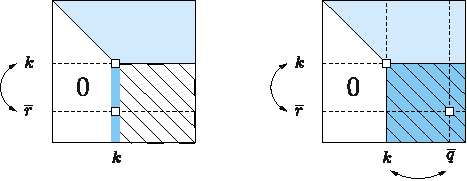
\includegraphics[width=.5\textwidth]{img/pivoting-by-rows-2.pdf}
\end{figure}